\documentclass[a4paper,12pt,titlepage]{article}
\usepackage{amsmath}
\usepackage[serbian]{babel}
\usepackage{verbatim}
\usepackage{graphicx}
\usepackage{latexsym}
\usepackage[margin=1in]{geometry}
\usepackage{color}
\usepackage{listings}
\usepackage[utf8]{inputenc}
\usepackage[T1]{fontenc}
\usepackage{currvita}
\usepackage{hyperref} 
\usepackage{float}

\newtheorem{definicija}{Definicija}[section]
\newtheorem{teorema}{Teorema}[section]
\renewcommand{\contentsname}{Sadr\v zaj}
\renewcommand{\refname}{Literatura}
\renewcommand{\mod}[1]{$mod$ ${#1}$}

\title{\Huge {\textbf{Obrada slike korišćenjem Guided filtra}}}
\author{\textbf{Autor:} Predrag Nikolić \and \textbf{Mentor:} Dejan Rančić}
\date{\today}

\begin{document}
\begin{center}
\large Univerzitet u Nišu \\ Elektronski fakultet
\end{center}

\begin{minipage}{\textwidth}
   \maketitle
\end{minipage}
\thispagestyle{empty}
\newpage

\tableofcontents
\thispagestyle{empty}
\newpage

\pagenumbering{arabic} 
\section{Obrada slike}%%%%%%%%%%%%%%%%%%%%%%%%%%

\subsection{Uvod}%%%%%%%%%%%%%%%%%%%%%%%

Računarska grafika je oblast računarstva koja se bavi obradom, stvaranjem i modeliranjem slika i video materijala, korišćenjem kompjutera. 
Ovaj izraz se obično odnosi na kompjuterski generisane podatke u vidu slike, koji su kreirani uz pomoć specijalizovanog softvera ili hardvera.
Ova oblast se odnosi na sve iz sveta kompjutera što nije prikazano tekstom ili zvukom.
Naučnici su počeli da se bave problemima iz računarske grafike još 60-ih, a danas ona obuhvata mnoge podoblasti i prožima mnoge druge
obalsti kako računarskih tako i drugih nauka. Neke od tema kojima se bavi računarska grafika su dizajn korisničkog interfejsa, spite grafika, vektorska grafika, 3D modeling itd. Možemo da zaključimo da se proučavanje računarske grafike, kao deo računarskih nauka, bavi metodima
za digitalnu obradu i manipulaciju visuelnim sadržajem. Iako se računarska grafika obično odnosi na tro-dimenzionalnu kompjutersku grafiku
takođe obuhvata i dvo-dimenzionalnu grafiku i obradu slike. 

Obrada slike je proces kod kojeg se slika ili video (koji je ustvari niz slika) obrađuju da bi se dobila izmenjena slika (video) ili skup karakteristika
ili nekih bitnih parametara. Slike se u obradi tretiraju kao signali pa se za njihovu obradu koriste metode iz oblasti obrade signala i razne matematičke operacije. Ova obalst je takođe usko povezana sa kompjuterskom vizijom i naravno kompjuterskom grafikom. Kada se kaže obrada slika obično se misli na digitalne slike, ali je takođe moguća i obrada optičkih i analognih slika. 

Digitalna slika može da se definiše kao funkcija $f(x, y)$, gde su $x$ i $y$ koordinate ravni. $x$ i $y$ predstavljaju koordinate piksela na slici. Pikseli su elementi od kojih je sastavljena slika. Obično $x$ predstavlja vrednost u odnosu na širinu slike, a $y$ u odnosu na visinu slike. Rezolucija slike se obično obeležava kao širina puta visina, izraženo u pikselima. Vrednost funkcije $f$ je intenzitet boje piksela na poziciji $(x, y)$. Intenzitet može da bude izražen kao jedna vrednost, ako je u pitanju crno bela slika, ili preko tri vrednosti ako je slika u boji. Postoje različiti načini za predstavaljanje slike u boji (Npr. RGB, CMYK, HSV itd.). Vrednosti funkcije $f$ kao i $x$ i $y$ su diskretne, jer je reč o digitalnoj slici. 

Čulo vida je nasloženije čulo čoveka i ima možda i najveću ulogu u čovekovoj precepciji okoline. Međutim no ono nije savršeno. Za razliku od ljudskog vida koji je limitiran vidljivim elektromagnetnim spektrom, u računarstvu imamo mogućnost da predstavimo ceo spektar i da se bavimo talasnim dužinama koje naše oko ne može da vidi. Obrada slika je složena oblast i prožima mnoge druge oblasti. Ne postoje jasne granice između obrade slike i oblasti kompjuterskog vida. Sama obrada slike može da bude deo sistema veštačke inteligencije za prepoznavanje lica ili nešto slično. Za obradu slike možemo da je porces koji na ulazu uzima sliku,   
vrši obradu i na izlazu se nalazi ponovo slika, ali u toku obrade takođe računa atribute te slike. 

Potreba za korišćenjem digitalnih slika javila se još 1920-tih godina u novinarstvu. Tada je prvi put slika poslana prekookenaski putem analognog kabla. Naravno prvi problemi koji su se javili tada imali su veze sa kvalitetom slike. Prvi sistemi su mogli da prenose crno bele slike, do 15 nijansi sive. Prvi kompjuteri koji su bili dovoljno moći da izvršavaju neku značajniju obradu slika javili su se 60-ih godina. Neke od prvih primena bile su vezane za poboljšanje slika iz svemira. Zatim je obrada slika počela da se koristi u medicini i astronomiji 70-ih godina, a i dan danas je bitna u tim oblastima.

\begin{figure}[ht!]
\centering
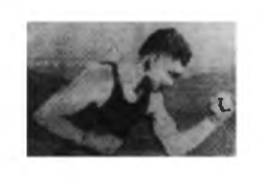
\includegraphics[width=75mm]{img/prvaPrenesenaSlika.png}
\caption{Digitalna slika koja je kreirana na osnovu kodirane trake 1921 godine}
\label{overflow}
\end{figure} 

U današnje vreme skoro da ne postoji oblast u kojoj se u nekoj meri ne koristi obrada slika. Jedna od najpoznatijih primena obrade slike je kreiranje i obrada rendgenskih slika (radiografija). Ona se najviše koristi u medicini ali postoje i druge primene. Primena postoji i za slike koje predstavljaju ultravioletnu boju. Ove slike se koriste u mikroskopiji. Postoje mnoge primene u svetu tehnologije kao što su izoštravanje slika, restauracija slika, prepoznavanje lica i objekata, prepoznavanje oblika. Takođe obrada slike se koristi u filmovima i medijima.  

Bitne komponente sistema za obradu slike su specijalizovan hardver za obradu slike, kao što su grafičke kartice, zatim kompjuter koji izvršava procese obrade slike i prikazuje rezultat. Takođe je bitan softver koji se koristi za obradu slike kao i komponente i metode za čuvanje velike količine podataka. Naravno možda i najbitniji komponenta je displej na kojem možemo da vidimo rezultat obrade slika.            

\subsection{Onsnovni procesi u obradi digitalne slike}%%%%%%%%%%%%%%%%%%%%%%%

Neki od osnovnih procesa i primena u obradi digitalne slike su sledeći. \emph{Pribavljanje slike} (eng. Image acquisition) se odnosi na to kako je slika nastala. Slika može da bude data u digitalnom obliku, a može da se zada i u analognom. Akvizicija slike uključuje predprocesiranje kao što je skaliranje i drugo. \emph{Poboljšanje slike} (eng. Image enhancement) je najprostiji ali i najkorišćeniji postupak u obradi slika. Cilj ovog procesa je da se na slici izraze bitni aspekti radi izučavanja parametra neke slike. Primene su različite (npr. izoštravanje ivica radi uočavanja detalja). \emph{Restauracija slike} (eng. Image restoration) je oblast koja se bavi poboljšanjem izgleda slike. Razlika između restauracije i poboljšanja je u tome što se tehnike za restauraciju oslanjaju na matematičke i probabilističke modele degradacije slike, dok se poboljšanje zasniva na subjektivnom osećaju čoveka. \emph{Obrada slika u boji} (eng. Color image processing) je oblast koja se bavi obradom slike u boji i artifaktima koje slike u boji donose u odnosu na obradu crno belih slika. \emph{Kompresija} (eng. Compression) se bavi tehnikama za kompresiju slike, radi smanjenja veličine slika, što je od velikog značaja za prenos i čuvanje podataka. \emph{Morfološka obrada slike} (eng. Morphological processing) se bavi alatima za ekstrakciju komponenti slika koji su pogodni za određenu reprezentaciju podataka koje slika nosi. \emph{Segmentacija} (eng. Segmentation) se bavi podelom slike na koezistentne delove ili objekte. \emph{Reprezentacija i deskripcija} (eng. Representation and description) kao što samo ime kaže se bavi predstavljanjem slike kako na ulazu tako i na izlazu nekog procesa obrade slike. I na kraju \emph{Prepoznavanje} (eng. Recognition) je proces u kojem se objektima dodeljuju labele odnosno imena na osnovu deskriptora, koji se mogu dobiti na osnovu slike. Svi ovi procesi mogu da koriste bazu znanja u kojoj se čuvaju bitne činjenice za svaki od procesa prilikom obrade slika. Postupci i osobine koje se javljaju na određenoj slici mogu da se jave ponovo. pa je čuvanje podataka o obradi veoma bitno.

U ovom radu ćemo se fokusirati na pribavljanje slike i poboljšanje slike.

\subsection{Pribavljanje slike}%%%%%%%%%%%%%%%%%%%%%%%

Iako je oblast digitalne obrade slika izgrađena na onovu matematičkih i probabilističkih formaulacija, pribavljanje slike je proces koji je određen na osnovu ljudskog čula vida. Slika se u digitalnom svetu pribavlja nasličan nači na koji čovek vidi, ondnosno kreira sliku u mozgu. Ljudski preceptor za vid je oko. Prozirni prednji delovi oka lome zrake svetlosti projektujući umanjenu i obrnutu sliku na fotosenzitivnu mrežnjaču gde se u specijalizovanim nervnim ćelijama ovbavlja pretvaranje slike u električne nervne impulse. Zrak se prelama u očnom sočivu, a deo oka odgovoran za prikupljanje slike je žuta mrlja, gde su nervene ćelije najgušće raspoređene. Pored žute mrlje se nalazi početag vidnog živca koji je neosetljiv na svetlo, pa se njegova projektcija u vidom polju naziva crna mrlja. Nervni impulsi kreirani u ćelijama se prenosu u mozak koji spaja slike iz oba oka i okreće obrnutu sliku čime se stvara osećaj vida u ljudskom mozgu.

Svetslost koju mi opažamo ima određeni intenzitet i boju. Ljudsko oko je sposobno da vidi samo deo elektromagnetnog spektra. Ono može da detektuje svetlost koja se u sprektru nalazi izmedju ultavioletne i infracrvene boje. Posto se svetlost tretira kao talas, boju odnosno deo spektra određuje talasna dužina. Talasna dužina se predstavalja kao odnos brzine svetlosti i frekvencije svetla $\lambda = c / \nu$. Energija koju nosi talas se računa se kao $E = h \nu$, gde je $h$ Plankova konstanta, a $\nu$ je frekvencija talasa. Ljudsko oko vidi svetlost talasne dužine između $0.4 * 10^{-6}m$ i $0.7 * 10^{-6}m$.

\begin{figure}[ht!]
\centering
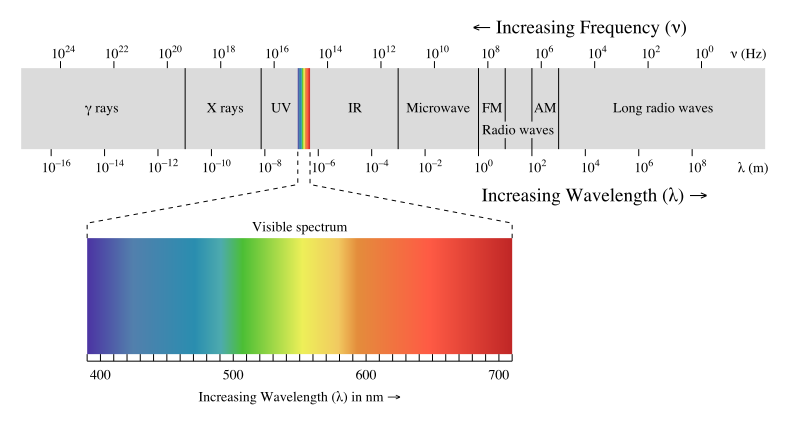
\includegraphics[width=120mm]{img/spektar.png}
\caption{Elektromagnetni spektar}
\label{overflow}
\end{figure} 

Slika se u digitalnom svetu generiše kao kombinacija osvetljenja prostora i reflektivne ili apsorbovane energije iz prostora scene za koju se pravi slika. Postoje raličiti tipovi senzora za akviziciju slika, ovde će biti opisan sistem sa senzorom u obliku 2-D niza (matrice). Senzor je sastavljen od elementata koji su raspoređeni u matrici. Svaki element je zadužen za prikupljanje svetlosti iz scene. U svakom elementu se beleži osveteljenje scene i tako se formira signal slike koji se kasnije dodatno obrađuje.

Pošto svetlost dolazi i kontinulanog prostora, vrednost signala koji nosi sliku će biti kontinualna. Da bi takav signal mogao da se obradi u računaru potrebno je da se taj signal digitalizuje. Digitalizaciju signala omogućuju semplovanje i kvantizacija. Semplovanje se odnosi na digitalizaciju koordinata piksela, odnosno određivanja mesta u prostoru. Kvantizacija se odonsi na digitalizaciju vrednosti amplitude signala. Pošto je slika skup određenog broja piksela od kojih svaki ima tačno određene koordinate u prostoru $(x, y)$, signal treba da se sampluje tako da svaki piksel bude popunjen jedinstvenom vrednošću. Vrednost amplitude signala je kontinualna, pa je kao takvu nemoguće sačuvati u računaru, zbog toga se uvodi kvantizacija gde se ta vrednost prevodi u diskretan prostor. Taj proces se naziva kvantizacija. Vrednost intenziteta piksela se obično predstavlja kao ceo broj izmedju 0 i 255. Postupak semplovanja i kvantizacije je bitan, jer od njega zavisi kvalitet i veličina podataka koje nosi signal slike. Ako je broj semplova ili kvantizacionih nivoa mali doći će do smanjenja kvaliteta slike, tj. slika neće biti verno prikazana. Međutim ako je broj  semplova ili kvantizacionih nivoa veliki broj podataka za čuvanje u memoriji će biti preveliki. U ovom postupku je bitno da se pronađe balans između ove dve stvari. U zavisnosti od potrebe će biti definisan broj semplova i kvantizacionih nivoa. Npr. nekada je bitnije da se sačuva što više slika, nego da slika bude precizna.  

Slika se u digitalnom svetu predstavlja kao $f(x, y)$, gde su $x$ i $y$ koordinate piksela na slici, a $f(x, y)$ je vrednost piksela u koordinatama $(x, y)$. 

\[
f(x, y)
=
\begin{bmatrix}
    f(0, 0) & f(0, 1) & f(0, 2) & \dots  & f(0, N - 1) \\
    f(1, 0) & f(0, 1) & f(1, 2) & \dots  & f(1, N - 1) \\
    \vdots & \vdots & \vdots & \ddots & \vdots \\
    f(M - 1, 0) & f(M - 1, 1) & f(M - 1, 2) & \dots  & f(M - 1, N - 1)
\end{bmatrix}
\]

, gde su N i M respektivno širina i visina slike.

Broj piksela slike se računa kao $b = M * N$, ako je slika crno bela, odnosno intenzitet piksela je prikazan kao jedna vrednost. Ako je u pitanju slika u boji onda se vrednost funkcije $f(x, y)$ predsavalja kao vektor vrednosti $[i_{1} i_{2} \dots i_{k}]$, gde je $k$ broj kanala, ondosno broj boja kojima je prikazana slika (najčešće 3 ako je u pitanju slika u boji). Tada se broj piksela računa kao $b = M * N * k$.

\subsection{Bitne relacije između piksela}%%%%%%%%%%%%%%%%%%%%%%%

Piksel $p$ sa koordinatama $(x, y)$ ima horizontalne i vertikalne susede $(x + 1, y)$, $(x - 1, y)$, $(x, y + 1)$, $(x, y - 1)$. Ovo se naziva 4-suseda piksela. Ako se dodaju dijagonalni susedi $(x + 1, y + 1)$, $(x - 1, y - 1)$, $(x + 1, y - 1)$, $(x - 1, y + 1)$ onda dobijamo 8-suseda piksela. Povezanost je osobina koja se dosta koristi u obradi slike. Ako su pikseli susedi i ako imaju istu vrednost ili vrednost iz istog podopsega mogućih vrednosti piksela onda su oni povezani. Putanja niz piksela koji su povezani na slici.

Postoje nekoliko načina za računanje distance između piksela. Ako imamo piksele $p$, $q$ i $z$ sa koordinatama $(x, y)$, $(s, t)$ i $(v, w)$, $D$ će biti mera distance ako važi: \\

a) $D(p, q) >= 0 (D(p, q) = 0 akko p = q)$,

b) $D(p, q) = D(q, p)$,

c) $D(p, z) <= D(p, q) + D(q, z)$.\\

Euklidska distanca: \\

\begin{center}
$D_{e}(p, q) = [ (x  - s)^{2} + (y - t)^{2} ]^{1/2}$
\end{center} 

Euklidska distanca nije baš pogodna za sliku koja ima diskretne vrendosti pa se za distancu koriste:\\

$D_{4}$ distanca 4-suseda:\\

\begin{center}
$D_{4}(p, q) = |x - s| + |y + t|$
\end{center} 

\[
\begin{bmatrix}
     &  & 2 &   &  \\
     & 2 & 1 & 2  &  \\
     2 & 1 & 0 & 1 & 2 \\
     & 2 & 1 & 2  &  \\
     &  & 2 &   &  \\
\end{bmatrix}
\].\\

$D_{8}$ distanca 8-suseda:\\

\begin{center}
$D_{8}(p, q) = max(|x - s|, |y + t|)$
\end{center} 

\[
\begin{bmatrix}
     2 & 2 & 2 & 2  & 2 \\
     2 & 1 & 1 & 1  & 2 \\
     2 & 1 & 0 & 1 & 2 \\
     2 & 1 & 1 & 1  & 2 \\
     2 & 2 & 2 & 2  & 2 \\
\end{bmatrix}
\].\\

\subsection{Osnovne operacije nad slikom u prostornom domenu}%%%%%%%%%%%%%%%%%%%%%%%

Glavni cilj poboljšanja slike je da se slika obradi na takav način, da krajnji rezultat zadovoljava odgovarajuću primenu. tehnika koja će da se koriti za obradu slike zavisi od konkretne primene i uslova koje rezultujuća slika treba da ispuni. Obrada slike se deli na dve kategorije: Obrada slike u prostornom domenu i obrada slike u frekvencijskom domenu. Prostorni domen se odonsi na ravan u kome se slika nalazi i metode koje izvršavaju operacije nad slikom u prostoru, dok se kod drugog tipa operacije izvršavaju nad slikom koja je predstavljena u obliku signala. U ovom radu će biti objašenjena obrada slike u prostornom domenu.

Kao što je navedeno obrada slike u prostronom domenu znači da se operacije izvršavaju nad pikselima. Ove procese možemo da označimo kao $g(x, y) = T[f(x, y)]$, gde je $f(x, y)$ početna slika, $g(x, y)$ obrađena slika, a $T$ je operator koji je definisan nad pikselima i njhovim susedima na slici $f$. Piksel $(x, y)$ i njegivi susedi prave pravougaonik, čiji je centar $(x, y)$, nad kojim se izvršava operacija $T$. Vrednost piksela $g(x, y)$ se računa kao vrednost piksela $f(x, y)$ i njegovih suseda, nad kojima se izvršavaju neke operacije. Ovaj proces se obično naziva konvolucija. Osnovni postupak obrade slike se izvršava tako što se za svaki piksel slike izvrši operacija nad tim pikselom i njegovim susedima i dobijena vrednost se dodeljuje tom pikselu. Postoje dva tipa dodele: dodela na mestu računanja kada se ista slika koristi za računanje i dodelu novih vrednosti i drugi tip dodele kod kojeg se dodela vrši na drugoj slici u piksel koji ima iste koordinate kao piksel kome se pristupa na slici koja se obrađuje.   

Ako vrednosti funkcija $f(x, y)$ i $g(x, y)$ predstavimo kao $r$ i $s$ respektivno, onda obradu slike možemo da predstavimo kao $s = T(r)$. U nastavku je da pregled nekih osnovnih transformacija nad slikom u prostornom domenu. Ove transformacije će biti predstavljene nad jednokanalnim slikama (slike čiji pikesli uzimaju samo jednu vrednost - nijansu sive boje). Što se tiče slika u boji postupak za ove transformacije je sličan. Transforamcije se ili vrše nad svakim kanalom nezavisno, ili se slika prevodi u sliku sa jednim kanalom (postoji više načina), pa se primenjuje određena transformacija.

Najosnovnija operacija koja može da se izvede nad slikom je negativ. Svaki piksel slike dobija inverznu vrednost u odnosu na svoju. Ako se vrednosti piksela kreću u granicama $[0, L - 1]$, rezultujuća vrednost se dobija kao $s = L - 1 - r$. Ova operacija se koristi na crno belim slikama koje su dominantno crne, a belom bojom su prikazani bitni podaci na slici, jer je lakse uočiti neke detalje.

\begin{figure}[ht!]
\centering
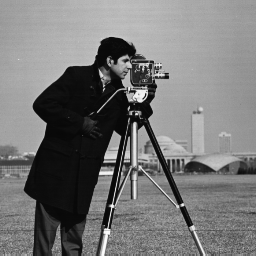
\includegraphics[width=60mm]{img/img.png}
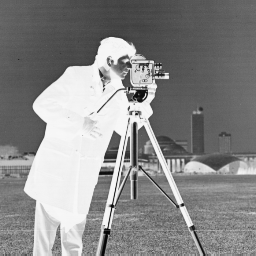
\includegraphics[width=60mm]{img/imgNegative.png}
\caption{Slika i njen negativ}
\label{overflow}
\end{figure} 

Nad slikom može da se primeni logaritamska operacija. $s = c*\log{1+ r}$. Ova operacija se koristi za izračunavanje spektra slike, što može da bude korisno za operacije koje se izvršavaju u kompleksnom domenu. Takođe nad slikom možemo da primenimo i stepene funkcije $s  = c*r^{\nu}$ ili $s = c*(r + \epsilon)^{\nu}$, gde su $c$ i $\nu$ pozitivne konstante i $\epsilon$ je konstanta. Ove opercije se koriste za gama korekciju. Jedna od najpozantijih primena je u tv uređajima koji su koriste katodne cevi. Takođe se koristi i za magnetnu rezonancu kako bi se pojačale boje i time izrazili detalji. 

\begin{figure}[ht!]
\centering
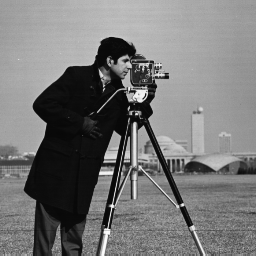
\includegraphics[width=60mm]{img/img.png}
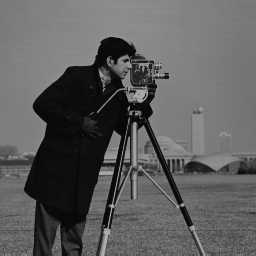
\includegraphics[width=60mm]{img/imgLog.png}
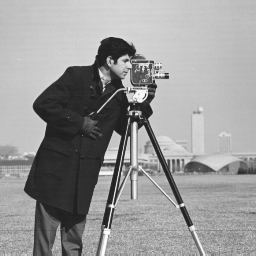
\includegraphics[width=60mm]{img/imgPow1.png}
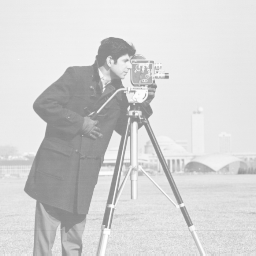
\includegraphics[width=60mm]{img/imgPow2.png}
\caption{Gore levo: Slika, gore desno: logaritamska transforamcija, dole levo: stepena transforamcija $c = 1 \nu = 0.6$, dole desno:  stepena transforamcija $c = 1 \nu = 0.3$}
\label{overflow}
\end{figure} 

Nasuprot predhodno navedena dva pristupa posoje i linearne transformacije. Nad slikom mogu da se izvode razne linearne funkcije. Neke od najkorićenijih su povećavaje kontrasta ili povećanje osvetljenja. Sve ove operacije imaju isti oblik $s = T(r)$, gde je T linearna transformacija, npr. menjanje osvetljenja slike može da se izrazi kao $s = r + c$ odnosno $s = r - c$, gde je $c$ konstanta u opsegu vrednosti koje uzimaju $s$ i $r$. 

Jedna od specifičnih obrada je obrada uz pomoć histograma. Histogram digitalne slike čiji pikseli uzimaju vrednosti iz $[0, L - 1]$ je diskretna funkcija $h(r_{k}) = n_{k}$, gde je $r_{k}$ k-ta vrednost u opsegu vrednosti koje uzimaju pikseli, a $n_{k}$ je broj piksela koji imaju tu vrednost. Obično se koristi noramlizovana f-ja $h(r_{k}) = n_{k}/n$, gde je n $max(n_{0}, n_{1}, ... , n_{L - 1})$, pa će sve vrednosti funkcije $h$ biti u opsegu $[0, 1]$. Histogrami mogu da se prikažu i grafički i oni nam ukazuju na to koje su nijanse zastupljene i kojoj meri na slici.  

\begin{figure}[ht!]
\centering
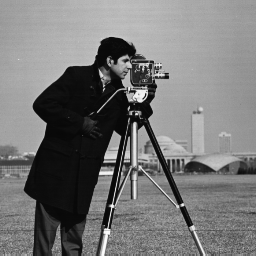
\includegraphics[width=60mm]{img/img.png}
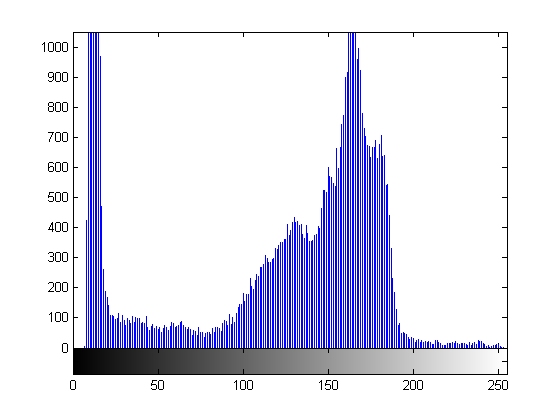
\includegraphics[width=60mm]{img/histImg.png}
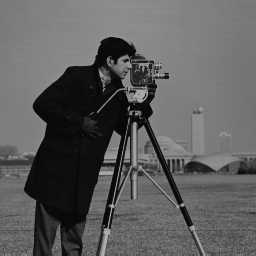
\includegraphics[width=60mm]{img/imgLog.png}
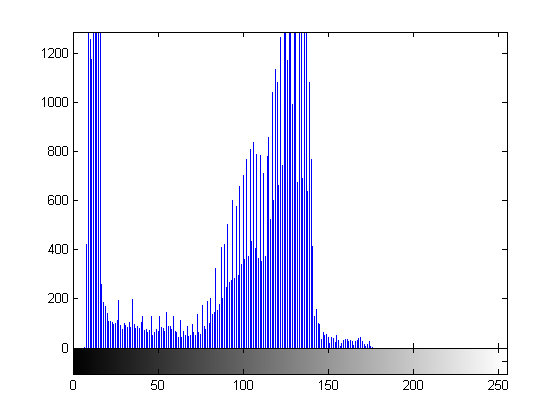
\includegraphics[width=60mm]{img/histImgLog.png}
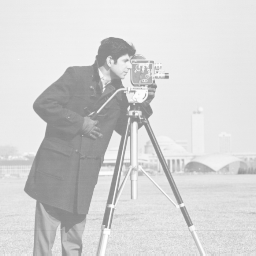
\includegraphics[width=60mm]{img/imgPow2.png}
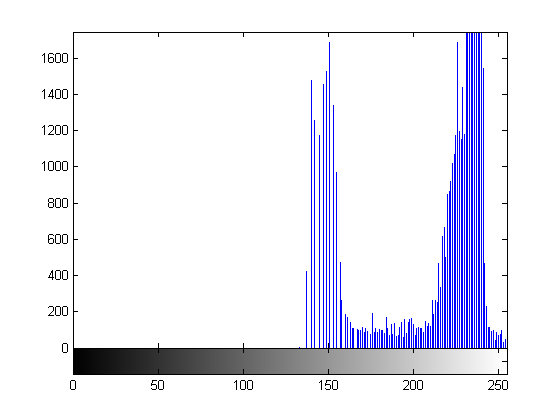
\includegraphics[width=60mm]{img/histImgPow2.png}
\caption{Histogram}
\label{overflow}
\end{figure} 

Obrada slike uz pomoć histograma se vrši tako što se izračuna histogram slike, nad njim se izvrši transformacija, a zatim pikseli na slici dobiju odgovarajuće vrednosti na osnovu transformisanog histograma. Nad histogramom mogu da se izvrše razne operacije u cilju pobolšanja slike.   
Jedna od operacija koja može da se izvrši uz pomoć histograma je histogramsko izjednačavanje. Cilj ovog postupka je da napravi uniformi histogram, tj. da na slici sve nijanse budu jednako zastupljene. Ovo je korisna transformacija ako je na slici dominiraju iste nijanse. Ako na slici dominirju određeni broj nijansi slika može da bude nejasna, izjednačavanjem odnosno uniformisanjem histograma dobijamo sliku koja ima zastupljene sve nijanse, što će dovesti do vizuelnog poboljšanja slike. Ovde ne zalazimo detaljno u aspekte obrade slike pomoću histograma, jer ona nije od važnosti za ovaj rad.

\begin{figure}[ht!]
\centering
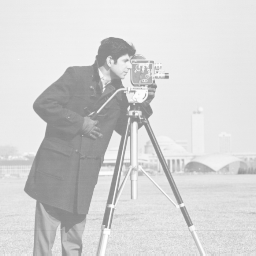
\includegraphics[width=60mm]{img/imgPow2.png}
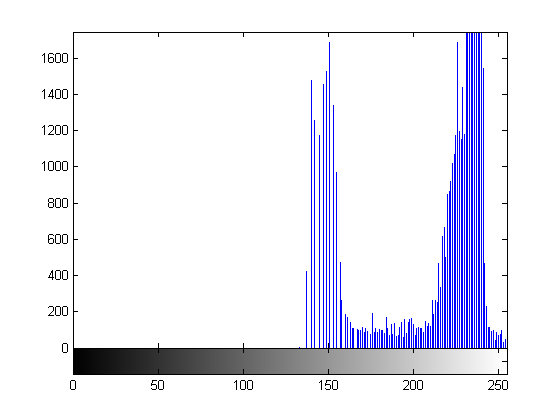
\includegraphics[width=60mm]{img/histImgPow2.png}
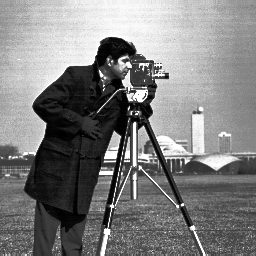
\includegraphics[width=60mm]{img/histEq.png}
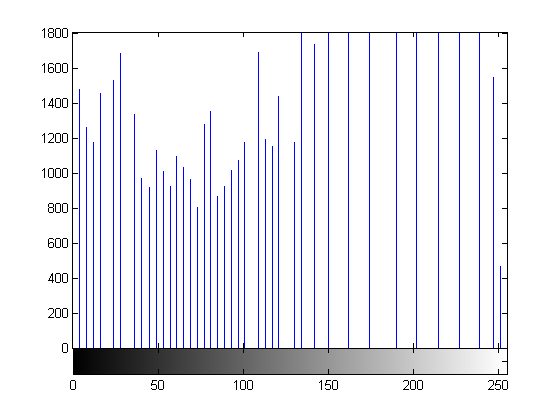
\includegraphics[width=60mm]{img/histEqhist.png}
\caption{Histogramsko izjendačavanje}
\label{overflow}
\end{figure}

Nad slikama možemo da primenimo i aritmetičke i logičke operacije. Logičke operacije AND, OR i NOT mogu da se primene nad slikama. AND operacija može da se koristi da bi se sa slike izvukao određeni region od značaja. Region može da se izvuče tako što će se primeniti AND operacija nad slikom i maskom. Maska je slika koja sadrži informaciju koji deo slike želimo da ostavimo. Maska se formira tako što se na mestima koje želimo da sadržimo stavaljmo maksimalnu vrednost koju uzimaju pikseli. Ako je opseg nijansi $[0, 1]$ onda je to 1, na svim ostalim mestima stavlja se 0. Rezultat ove operacije biće deo slike određen maskom. Na isti način se primenjuju i OR i NOT operacije. Logičke operacije su značajne za morfološku obradu slike koja je spomenuta kao jedna od oblasti kojima se bavi obrada slike. 

Nad slikama se često pirmenjuje operacija oduzimanja. Ako želimo da vidimo da li se dve slike razlikuju možemo da ih oduzmemo jednu od druge, što će da nam ukaze na razlike, jer će mesta gde su pikseli isti biti 0 tj crna a mesta gde ima ralike će biti predstavljena određenom nijansom. U ovu svrhu može da se koristi i deljenje. Sabiranje i množenje može da se koristi u svrhu dodavanja detalja na slici. 

\subsection{Osnovni pojmovi vezani za filtriranje u prostornom domenu}%%%%%%%%%%%%%%%%%%%%%%%

Kao što je ranije spomenuto prilikom obrade slike operacije se izvršavaju nad pikselom i njegovim susedima sa jedne strane i ogovarajućom podslikom sa druge. Ta pod slika nosi informacije o koje se koriste za filtriranje slike. Ta podslika (odnosno pravougaonih piksela) se naziva kernel ili prozor. Koncept filtriranja slike je uzet iz matematike ondnosno analize i matematički predstavljen taj proces je ustvari konvolucija $f * w$ gde je $f$ predstavlja sliku koja se filtrira, $w$ predstavlja kernel za filtriranje. Za svaki piksel slike koja se filtrira računa se nova vrednost uz pomoć kernela $w$ i odgovarajućeg piksela i njegovih suseda, iz slike. Ako imamo kernel oblika $3 x 3$ iračunavanje vrednosti piksela $(x, y)$ izgleda ovako\\

$R = w(-1, -1)f(x - 1, y - 1) + w(-1, 0)f(x - 1, y) + \dots + w(0, 0)f(x, y) + \dots + w(1, 0)f(x + 1, y) + w(1, 1)f(x + 1, y + 1)$.

\[
R
=
\begin{bmatrix}
     f(x - 1, y - 1) & f(x - 1, y) & f(x - 1, y + 1) \\
     f(x, y - 1) & f(x , y) & f(x, y + 1) \\
     f(x + 1, y - 1) & f(x + 1, y) & f(x + 1, y + 1) \\
\end{bmatrix}
.*
\begin{bmatrix}
     w(- 1, - 1) & w(- 1, 0) & w(- 1, 1) \\
     w(-0, - 1) & w(0, 0) & w(0, 1) \\
     w(1, - 1) & w(1, 0) & w(1, 1) \\
\end{bmatrix}
\].

Koeficijet kernela $w(0, 0)$ odgovara pikselu $f(x, y)$, što ukazuje na to da je maska centrirana oko piksela $(x, y)$. Obzirom da kernel mora da bude centriran oko jednog piksela, za kernel dimenzije $m x n$, važi da je $m = 2a + 1$ i $n = 2b + 1$, gde su $a$ i $b$ pozitivni celi brojevi. Najmanji kernel koji ima smisla je $3 x 3$ , a trivijalni slučaj predstavlja kernel $1 x 1$, koji se primenjuje samo kod osnovnih operacija. Generalno filtriranje slike $f$ dimenzija $M x N$, korišćenjem kernela $w$ veličine $m x n$ izrazom:\\

$g(x, y)  = \sum_{s = -a}^{a} \sum_{t = -b}^{b} w(s, t) f(x + s, y + t)$,\\

gde je $a = (m - 1) / 2, b = (n - 1) / 2$. Da bi se filtrirala cela slika potrebno je da se i zračuna vrednost $g(x, y)$ za svako $x \epsilon [0, M - 1]$ i za svako $y \epsilon [0, N - 1]$. 

Matrica kernela može da se obelži i ovako za primer kernela $3 x 3$:

\[
R
=
\begin{bmatrix}
     z_{1} & z_{2} & z_{3} \\
     z_{4} & z_{5} & z_{6} \\
     z_{7} & z_{8} & z_{9} \\
\end{bmatrix}
.*
\begin{bmatrix}
     w_{1} & w_{2} & w_{3} \\
     w_{4} & w_{5} & w_{6} \\
     w_{7} & w_{8} & w_{9} \\
\end{bmatrix}
\].

$R = w_{1}z_{1} + w_{2}z_{2} + \dots + w_{mn}f_{mn} = \sum_{i = 1}^{mn} w_{i}z_{i}$.\\

$w_{i}$ predstavlja vrednosti kernela, $z_{i}$ predstavlja vrednosti odgovarajućih piksela slike, a $m$ i $n$ predstavljaju dimenzije kernela.

Možemo da kažemo da se filtriranje obavlja tako što kernel prolazi kroz celu sliku. Ovaj pristup se koristi kako za linearne tako i za nelinerane filtre. Bitno je obratiti pažnju na piksele slike koji se nalaze uz ivicu slike. Ti pikseli nemaju sve susede pa oni moraju na neki načina da se dodele. To može da se reši na više različitih načina, a neki od uobičajnih su postavljanje vredosti tih suseda na 0 ili neku drugu konstantu ili uzimanje vrednosti simetričnih piksela u odnosu na piksel za koji se vrši konvolucija. 

Dva osnovna tipa filtera su filteri za uklanjanje šuma i zamućivanje slike koji se nazivaju smoothing filteri i filteri za izoštravanje slike, odnosno filteri za određivanje ivica ivica koji se nazivaju sharpening filteri. Pošto ne postoji tačan prevod za ove nazive dalje u radu se koriste imena smoothing i sharpening.

\subsection{Smoothing filtri(filtri za uklanjanje šuma)}

\subsection{Sharpening filtri(filtri za određivanje ivica)}

\subsection{Kombinovanje filtara}


\section{Guided filter}%%%%%%%%%%%%%%%%%%%%%%%%

\section{Primena}%%%%%%%%%%%%%%%%%%%%%%%%%%

\newpage
\addcontentsline{toc}{section}{Literatura}
\begin{thebibliography}{10}

\bibitem{ComputerGraphic}
\emph{\href{http://www.graphics.cornell.edu/online/tutorial/}{What is Computer Graphics?}},
Cornell University Program of Computer Graphics,
1998

\bibitem{introductiontoAI}
Rafael C. Gonzalez; Richard E. Woods,
\emph{\href{https://books.google.rs/books?id=8uGOnjRGEzoC&redir_esc=y}{Digital Image Processing}},
Prentice Hall,
2008.

\end{thebibliography}

\end{document}